\chapter{About this book}

Thanks a lot for purchasing a copy of \textit{Learn 2D iPhone Game Development
with SpriteBuilder, Cocos2D and Swift}. Over the last one and a half years I've
enjoyed working with \SB{} and \cocos{} while creating various tutorials for
\url{makeschool.com}. 

Why did I decide to write this book? While writing tutorials, I discovered my
passion for diving into details of the newly designed \cocos{} 3.0 API and
making my acquired knowledge available to a wide audience - many readers
have reached out to me, pointing to awesome projects that they have built based
on our tutorials.

After this initial success I created the first version of the official
documentation for \SB{} and \cocos{}:
\url{https://www.makeschool.com/docs/#!/cocos2d/1.2/overview}. As a developer
who has often struggled through adopting new frameworks, I truly believe that
good documentation is essential for the success of a product for software
developers.

This book fits neatly between the documentation and the tutorials we provide on
\url{makeschool.com}. It covers many aspects of the frameworks in depth while
providing you with a practical step-by-step guide on building an iPhone game that is available on the
App Store.

I hope this book helps you getting started with building amazing games!

\section{Who this book is for}
This book should be ideal for intermediate to advanced developers that have
previous experience with any object oriented programming language.

This book does not teach programming in general, or the \textit{Swift}
programming language from scratch! However, I don't assume you have any previous
knowledge in game programming.

I will briefly introduce \textit{Xcode}, the IDE we will be using, to make
sure you know how to run projects and use breakpoints. %TODO: make sure this is
%true

Besides that, this book focuses strongly on \SB{}, \cocos{} and 2D game
programming concepts. 

If you have experience in other programming languages, you will easily be able
to pick up Swift as you read through this book. Every once in a while we will
also discuss individual language features in more detail.

If you want a formal introduction to the Swift programming language, Apple's
book is the best reference:
\url{https://itunes.apple.com/us/book/swift-programming-language/id881256329?mt=11}

I've been burnt by reading books that try to cover too many different fields; I
wanted to write this book with a strong focus on its core topics.

\section{What this book covers}
This book covers most of the core features of \SB{} and \cocos{}, as well as
many concepts of 2D game programming. In many chapters I discuss details about
the \textit{Swift} programming language and also dive into aspects of good code
design. 

By reading this book you should get a very good idea of the \textit{big picture}
of 2D game development for iOS.

One large topic is not covered in this book: the \cocos{} physics engine. I
decided to leave it out, because it is a fairly large topic that is already very
well covered through Steffen Itterheim's \textit{Learn SpriteBuilder for iOS
Game Development} book. We also have an extensive physics based tutorial on the
Make School website:
\url{https://www.makeschool.com/tutorials/getting-started-with-spritebuilder/}.

I promise, after reading this book you will easily be able to pick up the
physics features of \SB{} and \cocos{} through our tutorial or the official
documentation.

%TODO: revisit after last edit
Here's a breakdown of the entire book by chapters:

\textbf{Chapter 1 - About this Book}\newline
This chapter discusses the structure of the book. It introduces different conventions and gives advice on how to get the most value out of the book.


\textbf{Chapter 2 - Introduction to SpriteBuilder and Cocos2D}\newline
Throughout this chapter you will build a first very simple game and learn about essential Cocos2D, SpriteBuilder and general 2D game programming concepts such as scene graphs, code connections and bounding boxes.


\textbf{Chapter 3 - A game with assets in SpriteBuilder}\newline
In this chapter you will start building the "Falling Food!" game on which you will work throughout the rest of the book. Chapter 3 will teach you all about asset handling with SpriteBuilder and Cocos2D. Learn how to integrate sprites and audio assets into your games. You will also learn how to use the update loop to implement object movement.


\textbf{Chapter 4 - User interaction and collision detection}\newline
Learn how to implement a drag and drop mechanism. You will also implement the core game mechanic of the game: catching objects based on their position. Since this game does not use the physics engine you will learn how to simulate physical behaviour with custom rendering code. You will also get to know details about the rendering order in Cocos2D.


\textbf{Chapter 5 - Scene graphs and node transforms}\newline
Learn how to incorporate a state machine into game development. You will also get to know details on affine transformations and how they are used to in Cocos2D to implement node hierarchies.


\textbf{Chapter 6 - User interfaces and implementing different game
modes}\newline The largest chapter in the book. Learn how to implement a level select screen using a scroll view. Leanr how to structure your game to support multiple game modes - without duplicating code. This chapter covers a variety of topics in UI programming and game programming patterns.


\textbf{Chapter 7 - Persisting Highscores}\newline
A brief chapter that explains how to build a simple Highscore system with NSUserDefaults.


\textbf{Chapter 8 - Effects and Animations}\newline
Learn how to use the powerfull CCEffects API to add lighting effects to your game! Dive deeper into SpriteBuilder's and Cocos2D's animation toolbox and polish the "Falling Food!" game.


\textbf{Chapter 9 - Where to go from here?}\newline
This chapter wraps up your learning experience. Find out about additional resources on SpriteBuilder and Cocos2D.

\section{About the author}
\begin{wrapfigure}{l}{0.20\textwidth}
    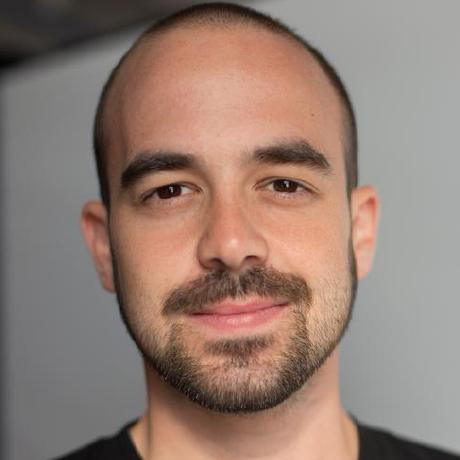
\includegraphics[width=0.18\textwidth]{images/Chapter1/benji.png}
\end{wrapfigure}
Hi! I'm Benjamin, the author of this book. I have four years of development experience on the iOS platform and two years of experience with Cocos2D.
I have written the original SpriteBuilder and Cocos2D documentation as well as many successful tutorials on makeschool.com. I regularly give talks on iOS development topics and love teaching passionate young developers at Make School. You can find me on Twitter, my personal blog or simply reach out to me via email: me@benjamin-encz.de.

\section{How to read this book}
I recommend to read this book in order when you are reading it for the first
time. In Chapter 3 we start working on a game that we complete throughout the
book - adding features chapter by chapter. By building this game you will learn
about \SB{} and \cocos{} concepts and see them unfold in an actual project.

Once you revisit this book you will have an understanding of how the project
evolves throughout the chapters. Then it will be easy to jump into individual
parts of the book and use them as a reference.

If you already know the basics of \cocos{} and \SB{} you can jump directly to
Chapter 4.

\section{Conventions in this book}
This book uses a few conventions to make reading it easier. 

\subsection{Info boxes}
Whenever I provide additional details on a topic that we just discussed, you
will see a special info box:
\begin{details}[An info box]
This information is interesting, but not essential.
\end{details}

\subsection{Action required}
This book is very \textit{hands on}. Whenever you are required to perform some
sort of action, you will see a gray bar as an indicator:

\begin{leftbar}
Follow the instructions provided in these blocks!
\end{leftbar}

The goal is to clearly separate the parts of the book that explain topics from
the parts that require you to do something.

\section{Source code}
All the source code shown throughout this book is available on a repository on
Github: \url{https://github.com/SpriteBuilder-Book/Code}. 

In that repository you'll find one project for each chapter in this book. Each
project contains the \SB{} project and source code for the specific progress of
one chapter. Whenever you get stuck you can look up the solution in that
repository.

\section{Getting involved}
I would love to have your feedback and hear about issues you found in this book.
You can report issues on this GitHub repository:
\url{https://github.com/SpriteBuilder-Book/Errata}. And you can email me at any
time with feedback or questions: me@benjamin-encz.de.